\documentclass[../rapport.tex]{subfiles}

\begin{document}

L'API est de type REST. Elle à été divisée en 3 endpoints (/user ; /wallet ; /financial\_product) correspondant chacun à un type de donnée pouvant être édité. 
Du à un manque de compréhension, nous n'avons pas utilisé les erreurs de la série 500 (problème serveur) dans le diagramme mais nous avons bien utilisé les erreurs de la série 400 correspondant à un problème dans la demande à l'API.

\begin{figure}[H]
    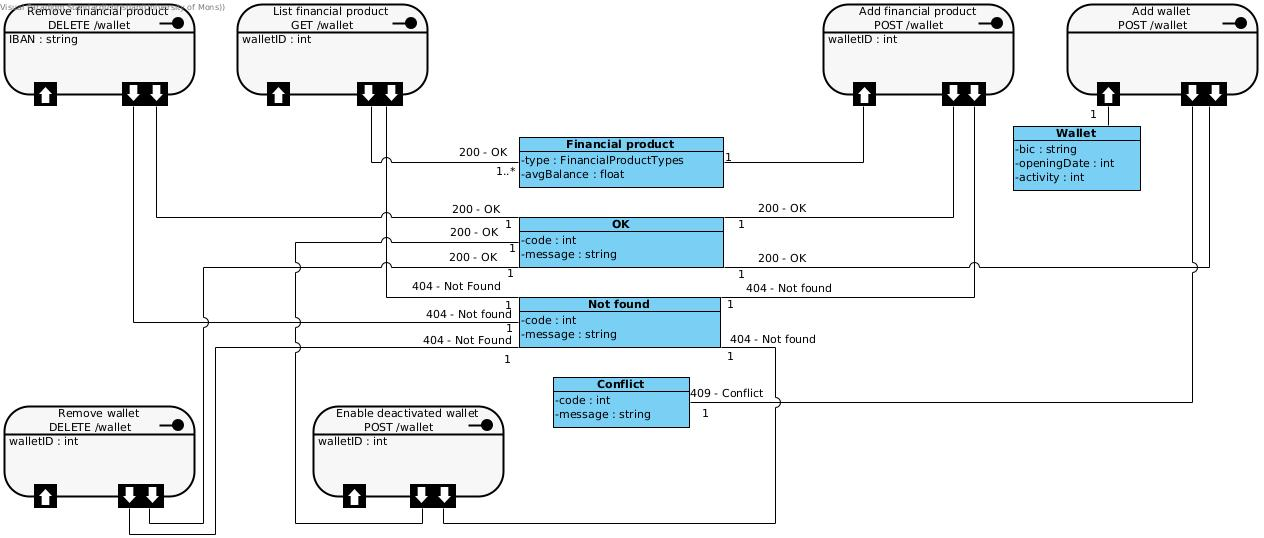
\includegraphics[scale=0.288]{ressources/photos_diagrammes/API/wallet.jpg}
\end{figure}

\begin{figure}[H]
    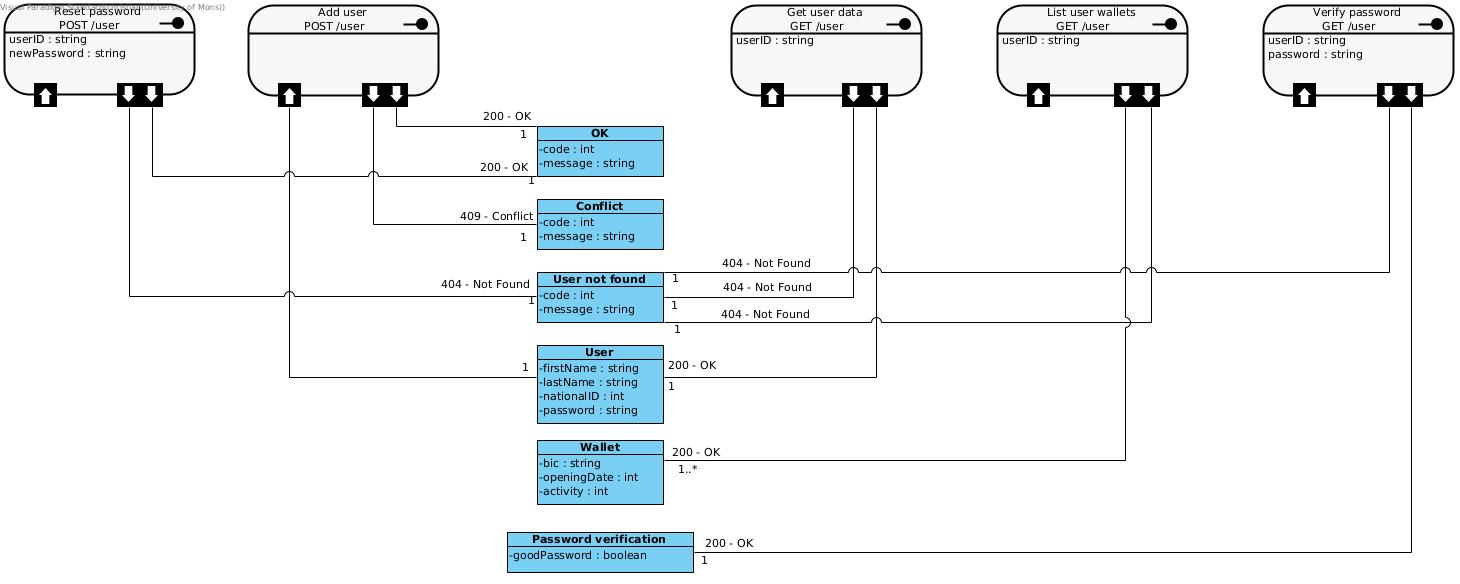
\includegraphics[scale=0.3]{ressources/photos_diagrammes/API/user.jpg}
\end{figure}

\begin{figure}[H]
    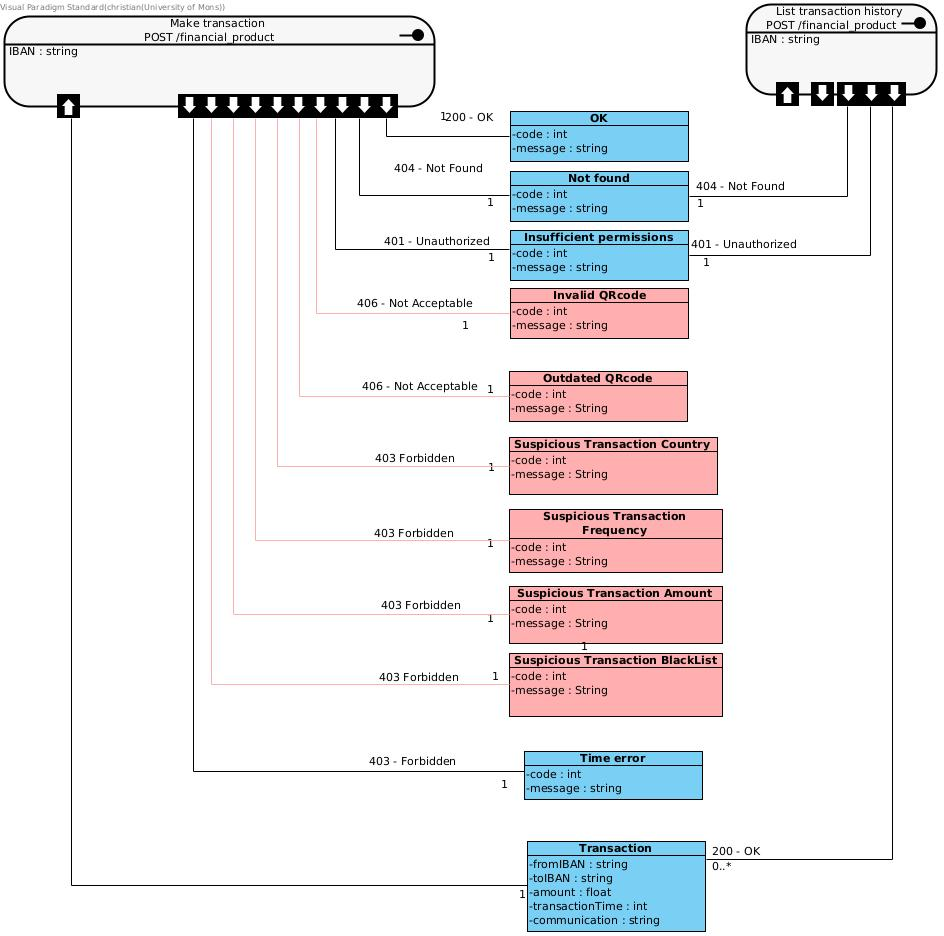
\includegraphics[scale=0.54]{ressources/photos_diagrammes/API/financial_product.jpg}
\end{figure}

\newpage

\end{document}
